% =====================================================================
%  Engineering Portfolio  - Mikko De Torres
%
%  Compile:  pdflatex portfolio.tex     (run it twice)
%
%  Design: full-bleed images, deep blue colour fields, and a title block
%  at the foot of every project sheet.
%
%  TO EDIT: go to the CONTENT section, well below.
%           Images live in images/<folder>/main.jpg
%           A missing image draws a coloured panel, so it always compiles.
% =====================================================================
\documentclass[11pt]{article}

\usepackage[a4paper,left=20mm,right=20mm,top=22mm,bottom=26mm,footskip=13mm]{geometry}
\usepackage[T1]{fontenc}
\usepackage{charter}
\usepackage[scaled=0.92]{helvet}
\usepackage{graphicx}
\usepackage{xcolor}
\usepackage{tikz}
\usepackage{array}
\usepackage{colortbl}
\usepackage{fancyhdr}
\usepackage{lastpage}
\usepackage[hidelinks]{hyperref}
\usepackage{parskip}
\usetikzlibrary{calc}

% -------- palette
\definecolor{deep}{HTML}{0E3A52}      % deep technical blue  - the mass colour
\definecolor{mid}{HTML}{17607F}       % mid blue
\definecolor{signal}{HTML}{E8912A}    % amber, used only as a marker
\definecolor{ink}{HTML}{15191B}
\definecolor{steel}{HTML}{58636B}
\definecolor{rule}{HTML}{C3CBCE}
\definecolor{panel}{HTML}{DDE5E9}
\definecolor{pale}{HTML}{F4F7F8}

\color{ink}
\setlength{\parindent}{0pt}
\linespread{1.06}

\pagestyle{fancy}
\fancyhf{}
\renewcommand{\headrulewidth}{0pt}
\renewcommand{\footrulewidth}{0pt}
\setlength{\headheight}{14pt}
\fancyfoot[L]{\sffamily\footnotesize\color{steel}Mikko De Torres  - Engineering portfolio}
\fancyfoot[R]{\sffamily\footnotesize\color{steel}\thepage\,/\,\pageref{LastPage}}

% -------- full-bleed band
% A band of image (or colour, if the image is missing) running edge to edge
% across the top of the page.
% #2 = image path   #3 = band height   #4 = caption if the image is missing
% Scales an image to fill a w x h box without stretching it.
% The extra is cropped off by the clip around it.
\newsavebox{\fillbox}
\newcommand{\fillimage}[3]{%
  \sbox{\fillbox}{\includegraphics[width=#2]{#1}}%
  \ifdim\dimexpr\ht\fillbox+\dp\fillbox\relax<#3
    \sbox{\fillbox}{\includegraphics[height=#3]{#1}}\fi
  \usebox{\fillbox}}

% #1 (optional) = move the image up or down inside the band, e.g. [10mm]
\newcommand{\bleedband}[4][0mm]{%
  \begin{tikzpicture}[remember picture,overlay]
    \IfFileExists{#2}{%
      \begin{scope}
        \clip (current page.north west) rectangle
              ($(current page.north east)+(0,-#3)$);
        \node[anchor=center,inner sep=0]
          at ($(current page.north)+(0,-0.5*#3)+(0,#1)$)
          {\fillimage{#2}{\paperwidth}{#3}};
      \end{scope}
    }{%
      \fill[panel] (current page.north west) rectangle
                   ($(current page.north east)+(0,-#3)$);
      \node[text=steel,font=\sffamily\small]
        at ($(current page.north)+(0,-0.5*#3)$) {#4};
      \fill[signal] ($(current page.north west)+(0,-#3)$) rectangle
                    ($(current page.north west)+(26mm,-#3-1.6mm)$);
    }
  \end{tikzpicture}%
  \vspace*{\dimexpr#3-22mm+8mm\relax}%
}

% -------- project heading
\newcommand{\projecttitle}[2]{%
  \noindent\textcolor{signal}{\rule{16mm}{2pt}}\par
  \vspace{3mm}
  {\sffamily\bfseries\fontsize{21}{24}\selectfont\color{deep} #1\par}
  \vspace{3mm}
  {\color{steel}\large #2\par}
  \vspace{5mm}
}

% -------- prose block
\newcommand{\detail}[2]{%
  {\sffamily\bfseries\small\color{deep} #1\par}
  \vspace{0.9mm}
  #2\par
  \vspace{3.4mm}
}

\newcommand{\todo}[1]{{\color{steel}\itshape #1}}

% -------- title block
\newcommand{\tbcell}[2]{%
  \begin{minipage}[t][13.2mm][t]{\linewidth}%
    \vspace{1.4mm}\hspace{2.2mm}%
    \begin{minipage}[t]{\dimexpr\linewidth-4.4mm\relax}
      {\color{white!72!deep}\fontsize{6.6}{8}\selectfont #1\par}
      \vspace{0.7mm}
      {\color{white}\fontsize{8.4}{9.6}\selectfont\raggedright\hyphenpenalty=10000\exhyphenpenalty=10000 #2\par}
    \end{minipage}%
  \end{minipage}}

\newcommand{\titleblock}[4]{%
  \vfill
  \noindent\begin{tikzpicture}
    \useasboundingbox (0,0) rectangle (\linewidth,-18.4mm);
    \fill[deep] (0,0) rectangle (\linewidth,-18.4mm);
    \node[anchor=north west,inner sep=0] at (0,-1.6mm)
      {\begin{minipage}{\linewidth}\sffamily
        \setlength{\arrayrulewidth}{0.4pt}\arrayrulecolor{white!35!deep}
        \begin{tabular}{@{}p{0.235\linewidth}|p{0.265\linewidth}|p{0.265\linewidth}|p{0.155\linewidth}@{}}
          \tbcell{Role}{#1} & \tbcell{Tools}{#2} &
          \tbcell{Context}{#3} & \tbcell{Year}{#4}
        \end{tabular}
        \arrayrulecolor{black}
      \end{minipage}};
  \end{tikzpicture}\par
  \rmfamily\normalsize
}

% =====================================================================
%                              CONTENT
% =====================================================================
\begin{document}

% -------- COVER
\thispagestyle{empty}
\begin{tikzpicture}[remember picture,overlay]
  % photograph band across the top half
  \IfFileExists{images/cover/main.jpg}{%
    \begin{scope}
      \clip (current page.north west) rectangle
            ($(current page.north east)+(0,-132mm)$);
      \node[anchor=center,inner sep=0] at ($(current page.north)+(0,-66mm)$)
        {\fillimage{images/cover/main.jpg}{\paperwidth}{132mm}};
    \end{scope}
  }{%
    \fill[panel] (current page.north west) rectangle
                 ($(current page.north east)+(0,-132mm)$);
    \node[text=steel,font=\sffamily\small]
      at ($(current page.north)+(0,-66mm)$)
      {[ images/cover/main.jpg  - you at the bench, or your best build ]};
  }
  % deep blue field below
  \fill[deep] ($(current page.north west)+(0,-132mm)$) rectangle
              (current page.south east);
  % amber marker straddling the seam
  \fill[signal] ($(current page.north west)+(22mm,-132mm)$) rectangle
                ++(34mm,-2.4pt);

  \node[anchor=north west,text=white,font=\sffamily\bfseries\fontsize{34}{38}\selectfont,align=left]
    at ($(current page.north west)+(22mm,-150mm)$)
    {Mikko De Torres};
  \node[anchor=north west,text=white!78!deep,font=\fontsize{13}{16}\selectfont,align=left]
    at ($(current page.north west)+(22mm,-165mm)$)
    {Mechatronics, robotics and AI engineer};
  \node[anchor=north west,text=white!62!deep,font=\sffamily\fontsize{10}{13}\selectfont,align=left]
    at ($(current page.north west)+(22mm,-174mm)$)
    {Mechanical design \quad CAD \quad 3D printing \quad Robotics \quad Machine learning};

  \node[anchor=south west,text=white!62!deep,font=\sffamily\fontsize{8.6}{12}\selectfont,align=left]
    at ($(current page.south west)+(22mm,22mm)$)
    {\todo{[ email ]} \quad\textbar\quad \todo{[ phone ]} \quad\textbar\quad Bauan, Batangas\\[1.4mm]
     \todo{[ portfolio site ]} \quad\textbar\quad \todo{[ LinkedIn ]} \quad\textbar\quad \todo{[ YouTube ]}};
\end{tikzpicture}
\clearpage

% -------- PROFILE
\thispagestyle{fancy}
\thispagestyle{fancy}
\vspace*{0mm}
\noindent\begin{minipage}[t]{0.38\linewidth}
  \vspace{0pt}
  \IfFileExists{images/portrait/main.jpg}{%
    \includegraphics[width=\linewidth,height=220mm,keepaspectratio]{images/portrait/main.jpg}%
  }{%
    
\begin{tikzpicture}
      \fill[panel] (0,0) rectangle (\linewidth,-220mm);
      \node[text=steel,font=\sffamily\small] at (0.5\linewidth,-110mm)
        {[ portrait photo ]};
    \end{tikzpicture}%
  }
\end{minipage}%
\hspace{5mm}%
\begin{minipage}[t]{0.57\linewidth}
  \vspace{0pt}
  \noindent\textcolor{signal}{\rule{16mm}{2pt}}\par
  \vspace{3mm}
  {\sffamily\bfseries\fontsize{18}{22}\selectfont\color{deep}
   Engineer, and the person who explains it\par}
  \vspace{4mm}

  I design mechanical systems and then build them. My work runs from CAD modelling and
  3D printing through electronics, control code and testing, and into the documentation
  and video that explain it.

  \vspace{2.5mm}
  Seven years in industry as a maintenance and automation engineer, then seven teaching
  robotics, control systems and machine learning at Batangas State University. I am
  finishing an MS in Artificial Intelligence on motion planning for six-axis manipulators.

  \vspace{5mm}
  {\sffamily\bfseries\small\color{deep}What I bring to a team\par}
  \vspace{1.5mm}
  A working knowledge of the whole loop , design it, build it, wire it, program it,
  test it, then document it well enough that someone else can pick it up. Teaching made
  the last part second nature.

  \vspace{4mm}
  {\sffamily\bfseries\small\color{deep}Mechanical design and CAD\par}
  \vspace{1.5mm}
  SolidWorks, Onshape, AutoCAD. Designed the structure and folding mechanism of a
  DOST-funded solar power station, built and deployed as a working prototype.

  \vspace{4mm}
  {\sffamily\bfseries\small\color{deep}Electronics and code\par}
  \vspace{1.5mm}
  Arduino, ROS, C++, Python, MATLAB. Built a 3-DOF manipulator controlled through ROS
  and Arduino, with the kinematics solved in Python.

  \vspace{4mm}
  {\sffamily\bfseries\small\color{deep}Teaching and documentation\par}
  \vspace{1.5mm}
  Robotics 1 and 2, control systems, machine learning and data science, microprocessors,
  physical systems modelling, basic workshop and machining. I run a YouTube channel on
  the same subjects.

  \vspace{4mm}
  {\sffamily\bfseries\small\color{deep}Education\par}
  \vspace{1.5mm}
  BS Mechatronics Engineering, 2012. MS Artificial Intelligence, in progress. Both at
  Batangas State University.
\end{minipage}
\clearpage

% -------- PROJECT 1
\bleedband[-12mm]{images/solar-station/deployed.jpg}{60mm}
          {[ the deployed unit in the field ]}
\vspace{-24mm}

\projecttitle{Collapsible solar power station for farms}
             {A portable, foldable solar power unit for farm use, funded by DOST-TAPI
              and built to a working prototype.}

\detail{The problem}{\todo{What farms could not do without this, and why existing solar
units did not fit  - weight, cost, transport, setup time?}}

\detail{What I built}{The mechanical structure and the folding mechanism, modelled in
SolidWorks. The unit carries photovoltaic panels and a battery storage unit, and
collapses so one team can move, deploy and store it without special equipment.}

\vspace{3mm}
\noindent\begin{minipage}[t]{0.30\linewidth}
  \IfFileExists{images/solar-station/main.jpg}{%
    \includegraphics[width=\linewidth]{images/solar-station/main.jpg}%
  }{}
  \par\vspace{1.5mm}
  {\sffamily\footnotesize\color{steel}SolidWorks  - open}
\end{minipage}%
\hspace{0.025\linewidth}%
\begin{minipage}[t]{0.30\linewidth}
  \IfFileExists{images/solar-station/folded-front.jpg}{%
    \includegraphics[width=\linewidth]{images/solar-station/folded-front.jpg}%
  }{}
  \par\vspace{1.5mm}
  {\sffamily\footnotesize\color{steel}SolidWorks  - front}
\end{minipage}%
\hspace{0.025\linewidth}%
\begin{minipage}[t]{0.30\linewidth}
  \IfFileExists{images/solar-station/folded-back.jpg}{%
    \includegraphics[width=\linewidth]{images/solar-station/folded-back.jpg}%
  }{}
  \par\vspace{1.5mm}
  {\sffamily\footnotesize\color{steel}SolidWorks  - back}
\end{minipage}
\vspace{4mm}

\detail{How}{SolidWorks for the structure and mechanism, then fabrication drawings. I
also produced the brochure and the instruction materials the users received.}

\titleblock{Mechanical design lead}{SolidWorks, fabrication drawings}
           {DOST-TAPI funded project}{2023-24}
\clearpage

% -------- PROJECT 2
\bleedband{images/robot-arm-6dof/pick-place.jpg}{65mm}
          {[ pick and place in the lab ]}
\vspace{-20mm}

\projecttitle{3-DOF to 6-DOF robot arm kit}
             {A modular robot arm, 3D printed and assembled from three to six axes
              depending on the configuration  - a teaching platform my students learn
              kinematics on.}

\vspace{2mm}
\noindent\begin{minipage}[t]{0.22\linewidth}
  \includegraphics[width=\linewidth]{images/robot-arm-6dof/main.jpg}
  \par\vspace{1mm}{\sffamily\footnotesize\color{steel}CAD - view 1}
\end{minipage}%
\hspace{0.02\linewidth}%
\begin{minipage}[t]{0.22\linewidth}
  \includegraphics[width=\linewidth]{images/robot-arm-6dof/cad2.jpg}
  \par\vspace{1mm}{\sffamily\footnotesize\color{steel}CAD - view 2}
\end{minipage}%
\hspace{0.02\linewidth}%
\begin{minipage}[t]{0.22\linewidth}
  \includegraphics[width=\linewidth]{images/robot-arm-6dof/gripper.jpg}
  \par\vspace{1mm}{\sffamily\footnotesize\color{steel}Gripper design}
\end{minipage}%
\hspace{0.02\linewidth}%
\begin{minipage}[t]{0.22\linewidth}
  \includegraphics[width=\linewidth]{images/robot-arm-6dof/assembled.jpg}
  \par\vspace{1mm}{\sffamily\footnotesize\color{steel}Assembled arm}
\end{minipage}
\vspace{3mm}

\detail{What I built}{A six-axis arm designed in SolidWorks and 3D printed. Assembled
with servo motors, a custom gripper, and an Arduino-based controller. Used in robotics
classes for kinematics, pick-and-place and path planning demonstrations.}

\detail{How}{3D printed parts, SolidWorks, Arduino, servo motors. Competed and
demonstrated at robotics events.}

\titleblock{Built and integrated}{SolidWorks, 3D printing, Arduino}
           {Robotics teaching platform}{2023-24}
\clearpage

% -------- PROJECT 3
\bleedband{images/ros-manipulator/rviz.jpg}{65mm}
          {[ RViz MoveIt simulation ]}
\vspace{-20mm}

\projecttitle{3-DOF articulated manipulator on ROS and Arduino}
             {A three-axis arm where the mechanical build, the electronics and the
              control software all had to meet.}

\noindent\begin{minipage}[t]{0.48\linewidth}
  \includegraphics[width=\linewidth]{images/ros-manipulator/actual.jpg}
  \par\vspace{1mm}{\sffamily\footnotesize\color{steel}Actual Arduino robot}
\end{minipage}%
\hspace{0.04\linewidth}%
\begin{minipage}[t]{0.48\linewidth}
  \includegraphics[width=\linewidth]{images/ros-manipulator/rviz.jpg}
  \par\vspace{1mm}{\sffamily\footnotesize\color{steel}MoveIt simulation in RViz}
\end{minipage}
\vspace{4mm}

\detail{What I built}{The manipulator itself, with real-time control written in C++
under ROS and the kinematics solved in Python for motion planning. Simulated in MoveIt
for path planning and visualized in RViz.}

\detail{How}{ROS for the control layer, Arduino for the hardware interface, C++ for the
real-time loop, Python for the kinematics, MoveIt for motion planning.}

\titleblock{Built and programmed}{ROS, Arduino, C++, Python, MoveIt}{Robotics laboratory}{2023-24}
\clearpage

% -------- PROJECT 4
\bleedband{images/weld-vision/main.jpg}{72mm}
          {[ weld classification results ]}
\vspace{-20mm}

\projecttitle{Weld inspection by machine vision}
             {A vision system that classifies weld quality on stainless steel from HDR
              camera images - contamination, burn-through, or good weld.}

\detail{What I built}{A full classification pipeline in Python that takes HDR camera
images of a weld and classifies the defects. The dataset includes contamination,
burn-through and good weld classes, captured under HDR imaging to hold detail across
the bright arc and dark surrounding metal.}

\detail{How}{Transfer learning on a pre-trained VGG16 network for feature extraction,
then retrained for weld defect classification. HDR imaging holds detail across the
bright and dark parts of the weld.}

\titleblock{Full pipeline}{Python, HDR imaging, VGG16, transfer learning}{Machine vision project}{2023-24}
\clearpage

% -------- PROJECT 5
\bleedband{images/matlab-sims/scara_v3.jpg}{65mm}
          {[ SCARA V3 simulation ]}
\vspace{-20mm}

\projecttitle{Manipulator simulations in MATLAB}
             {Simulations of every major manipulator type, written for the robotics
              courses I teach.}

\noindent\begin{minipage}[t]{0.18\linewidth}
  \includegraphics[width=\linewidth]{images/matlab-sims/cartesian_jv.jpg}
  \par\vspace{1mm}{\sffamily\fontsize{6.5}{8}\selectfont\color{steel}Cartesian}
\end{minipage}%
\hspace{0.015\linewidth}%
\begin{minipage}[t]{0.18\linewidth}
  \includegraphics[width=\linewidth]{images/matlab-sims/cylindrical_jv.jpg}
  \par\vspace{1mm}{\sffamily\fontsize{6.5}{8}\selectfont\color{steel}Cylindrical}
\end{minipage}%
\hspace{0.015\linewidth}%
\begin{minipage}[t]{0.18\linewidth}
  \includegraphics[width=\linewidth]{images/matlab-sims/spherical_jv.jpg}
  \par\vspace{1mm}{\sffamily\fontsize{6.5}{8}\selectfont\color{steel}Spherical}
\end{minipage}%
\hspace{0.015\linewidth}%
\begin{minipage}[t]{0.18\linewidth}
  \includegraphics[width=\linewidth]{images/matlab-sims/articulated_jv.jpg}
  \par\vspace{1mm}{\sffamily\fontsize{6.5}{8}\selectfont\color{steel}Articulated}
\end{minipage}%
\hspace{0.015\linewidth}%
\begin{minipage}[t]{0.18\linewidth}
  \includegraphics[width=\linewidth]{images/matlab-sims/scara_jv.jpg}
  \par\vspace{1mm}{\sffamily\fontsize{6.5}{8}\selectfont\color{steel}SCARA}
\end{minipage}
\vspace{4mm}

\detail{What I built}{Simulations of the Cartesian, cylindrical, spherical, articulated
and SCARA manipulator types, plus a 6-DOF SCARA V3, each covering kinematics, dynamics
and control. Used in Robotics 1 and 2 classes for third-year students.}

\detail{How}{MATLAB with Peter Corke's Robotics Toolbox. Each simulation includes a
Teach pendant interface for interactive joint control and end-effector position readout.}

\titleblock{Wrote all simulations}{MATLAB, Robotics Toolbox}
           {Robotics 1 and 2 teaching material}{2022-24}
\clearpage


% -------- CAPSTONE 1
\bleedband{images/capstone-robots/cad1.jpg}{62mm}
          {[ Cartesian CNC robot CAD ]}
\vspace{-20mm}

\projecttitle{Robot design and simulation}
             {Manipulator and machine projects I designed, modelled and programmed
              with student teams at the Mechatronics and Robotics Laboratory.}

\noindent\begin{minipage}[t]{0.23\linewidth}
  \includegraphics[width=\linewidth]{images/capstone-robots/cad2.jpg}
  \par\vspace{1mm}{\sffamily\fontsize{6.5}{8}\selectfont\color{steel}Cartesian CNC - CAD}
\end{minipage}%
\hspace{0.02\linewidth}%
\begin{minipage}[t]{0.23\linewidth}
  \includegraphics[width=\linewidth]{images/capstone-robots/flowchart.jpg}
  \par\vspace{1mm}{\sffamily\fontsize{6.5}{8}\selectfont\color{steel}Data integration}
\end{minipage}%
\hspace{0.02\linewidth}%
\begin{minipage}[t]{0.23\linewidth}
  \includegraphics[width=\linewidth]{images/capstone-robots/front.jpg}
  \par\vspace{1mm}{\sffamily\fontsize{6.5}{8}\selectfont\color{steel}Kinematics - front}
\end{minipage}%
\hspace{0.02\linewidth}%
\begin{minipage}[t]{0.23\linewidth}
  \includegraphics[width=\linewidth]{images/capstone-robots/top.jpg}
  \par\vspace{1mm}{\sffamily\fontsize{6.5}{8}\selectfont\color{steel}Kinematics - top}
\end{minipage}
\vspace{3mm}

\detail{Cartesian CNC robot - digital twin}{Geometric design in SolidWorks and
the programmed digital twin integrated with LinuxCNC. Includes kinematics, data
integration pipeline and engineering drawings. May 2023.}

\detail{3-DOF RRP SCARA manipulator}{Design and development of the machine elements,
and the robot programming. May 2024.}

\detail{5-DOF articulated manipulator - LinuxCNC integration}{Real-time testing and
LinuxCNC integration for the motors and the digital twin. May 2024.}

\titleblock{Design and programming}{SolidWorks, LinuxCNC, MATLAB}
           {Robotics Laboratory}{2023-24}
\clearpage

% -------- 6-DOF MANIPULATOR IN COPPELIASIM
\bleedband[-26mm]{images/coppeliasim-6dof/path.jpg}{65mm}
          {[ 6-DOF arm following a path in CoppeliaSim ]}
\vspace{-20mm}

\projecttitle{6-DOF manipulator in CoppeliaSim}
             {A six-axis arm I designed in SolidWorks, checked for stress, and
              programmed to move in a CoppeliaSim simulation.}

\vspace{2mm}
\noindent\begin{minipage}[t]{0.32\linewidth}
  \begin{minipage}[t][40mm][c]{\linewidth}\centering\includegraphics[width=\linewidth,height=40mm,keepaspectratio]{images/coppeliasim-6dof/cad.jpg}\end{minipage}
  \par\vspace{1mm}{\raggedright\sffamily\footnotesize\color{steel}SolidWorks model\par}
\end{minipage}%
\hspace{0.02\linewidth}%
\begin{minipage}[t]{0.32\linewidth}
  \begin{minipage}[t][40mm][c]{\linewidth}\centering\includegraphics[width=\linewidth,height=40mm,keepaspectratio]{images/coppeliasim-6dof/stress.jpg}\end{minipage}
  \par\vspace{1mm}{\raggedright\sffamily\footnotesize\color{steel}Stress study of the base\par}
\end{minipage}%
\hspace{0.02\linewidth}%
\begin{minipage}[t]{0.32\linewidth}
  \begin{minipage}[t][40mm][c]{\linewidth}\centering\includegraphics[width=\linewidth,height=40mm,keepaspectratio]{images/coppeliasim-6dof/sim.jpg}\end{minipage}
  \par\vspace{1mm}{\raggedright\sffamily\footnotesize\color{steel}Model in CoppeliaSim\par}
\end{minipage}
\vspace{5mm}

\noindent\begin{minipage}[t]{0.62\linewidth}
\detail{What I built}{A six-axis arm modelled in SolidWorks, with a static stress
study on the base under load. I brought the model into CoppeliaSim and programmed its
forward and inverse kinematics, so the arm follows a set path.}

\detail{How}{Press play and the arm starts moving. While it moves, the simulation
plots the tool position and the joint speeds live. SolidWorks for the design and
stress study, CoppeliaSim for the simulation.}
\end{minipage}%
\hspace{0.06\linewidth}%
\begin{minipage}[t]{0.32\linewidth}
  \vspace{0pt}\centering
  \includegraphics[width=\linewidth,height=72mm,keepaspectratio]{images/coppeliasim-6dof/flowchart.jpg}
  \par\vspace{1mm}{\raggedright\sffamily\footnotesize\color{steel}Program flow\par}
\end{minipage}

\titleblock{Design and simulation}{SolidWorks, CoppeliaSim}
           {Robotics Laboratory}{2024}
\clearpage

% -------- TEACHING
\bleedband{images/youtube/main.jpg}{74mm}
          {[ channel screenshot, or two or three thumbnails ]}

\projecttitle{Teaching, filming and open material}
             {The engineering is only half of it. I also make the material that explains
              it.}

\detail{Mechatronics and Robotics Engineering on YouTube}{I script, film and edit
technical videos on robotics, data science in Excel, Git and GitHub, and basic workshop
and machining.}

\detail{Course repositories}{\textbf{Robotics\_MEXE\_3rdYearCourse}  - kinematics,
control algorithms and simulation tasks for Robotics 1 and 2.\\
\textbf{MexEE402\_AI}  - data science, machine learning and model productionization.}

\detail{Print documentation}{Brochure and instruction materials for the solar power
station, written for the farmers who would use it.}

\titleblock{Author and presenter}{Video, GitHub, technical writing}
           {Public teaching material}{2019-present}
\clearpage

% -------- CLOSING
\thispagestyle{empty}
\begin{tikzpicture}[remember picture,overlay]
  \fill[deep] (current page.north west) rectangle (current page.south east);
  \fill[signal] ($(current page.north west)+(22mm,-72mm)$) rectangle ++(34mm,-2.4pt);

  \node[anchor=north west,text=white,font=\sffamily\bfseries\fontsize{25}{29}\selectfont,align=left]
    at ($(current page.north west)+(22mm,-88mm)$)
    {Let's build something.};

  \node[anchor=north west,text=white!78!deep,font=\fontsize{11.5}{16}\selectfont,align=left,
        text width=118mm]
    at ($(current page.north west)+(22mm,-104mm)$)
    {If any of this is close to what you are working on, I would be glad to talk it
     through.};

  \node[anchor=north west,text=white!62!deep,font=\sffamily\fontsize{9.4}{15}\selectfont,align=left]
    at ($(current page.north west)+(22mm,-134mm)$)
    {\todo{[ email ]}\\ \todo{[ phone ]}\\ \todo{[ portfolio site ]}\\
     \todo{[ LinkedIn ]}\\ \todo{[ YouTube ]}\\ \todo{[ GitHub ]}};
\end{tikzpicture}

\end{document}
